\section{Parametrisierte Algorithmen}

\begin{takeaway}
    \item Parametrisierter Algorithmus, fpt
    \item Standard-Parametrisierung
    \item Kernbildung
    \item (Sichere) Datenreduktionsregel
    \item Kronenzerlegung
    \item Tiefenbeschränkte Suchbäume
    \item Iterative Kompression
    \item Baumzerlegung, Baumweite; bramble, bramble number
    \item Klasse W[1]
    \item Probleme: Edge Clique Cover, Cluster Editing, Steinerbaum, VCP via Baumweite
\end{takeaway}

\paragraph{Idee}
Verallgemeinerung von pseudopolynomiellen Algorithmen:
Laufzeit hängt von der Eingabegrösse nur polynomiell ab, aber darf beliebig gross 
werden in der Grösse eines Parameters.
Partitionierung in Problemklassen entlang des Parameters.

\paragraph{Parametrisierung}
Sei $U$ ein Entscheidungsproblem, $L$ die Sprache der Eingaben.
$\Par: L \mapsto \N$ ist eine \emph{Parametrisierung} von $U$ falls gilt:
\begin{enumerate}[label=(\roman*)]
    \item $\Par$ ist in Polynomzeit berechenbar
    \item Für unendlich viele $k \in \N$ ist die Parameter-$k$-Menge für $U$
    $$ Set_U(k) := \{ I \in L \st \Par(I) = k \} $$ unendlich.
    Dies stellt sicher dass $\Par$ nichttrivial ist, z.B. nicht etwa $\Par(I) = |I|$.
    In anderen Worten, für jeden Parameterwert soll es beliebig viele Probleminstanzen geben.
\end{enumerate}
Ein Algorithmus $\A$ heisst \emph{$\Par$-paremetrisierter Polynomzeit-Algorithmus} für $U$ falls gilt:
\begin{enumerate}[label=(\roman*)]
    \item $\A$ löst $U$
    \item $ \exists \text{ Polynom } p \; \exists \text{ (berechenbare) Funktion } f : \N \mapsto \N$
    so dass $\forall I \in L$:
    $$\Time_\A(I) \leq f \big( \Par(I) \big) \cdot p(|I|) $$
\end{enumerate}

Falls ein solcher Algorithmus existiert, dann heisst $U$ \emph{fixed-parameter-tractable 
bezüglich $\Par$}.
$\A$ wird auch \emph{fpt-Algorithmus für $U$ bezüglich $\Par$} genannt und läuft in \emph{fpt-Zeit}.

\underline{Beispiel:} Sei $U$ ein Zahlproblem und sei $Val(I) := \max \{ |x_i| \}$.
Es gilt $\text{max-int}(I) \leq 2^{Val(I)}$. Somit ist ein pseudopolynomieller 
Algorithmus $\A$ für $U$ auch ein $Val$-Parametrisierter Algorithmus für $U$.

\paragraph{Ansätze}
Die \emph{Standard-Parametrisierung} wählt als Parameter die Grösse der gewünschten 
Lösung (z.B. Grösse des VCs).
Die \emph{Strukturelle Parametrisierung} wählt eine bestimmte Eigenschaft der Eingabe 
(z.B. maximaler Knotengrad).
Andere Ansätze betrachten wir im Folgenden.


\subsection{Kernbildung}

\paragraph{Idee}
Polynomielles Preprocessing, Datenreduktion, um die Instanz auf einen \emph{Kern} zu verkleinern,
der in seiner Grösse nur noch vom Parameter abhängt.
Diesen Kern dann mit bekannten Algorithmen (oder brute force) lösen.

\paragraph{Kernbildung (kernelisation)}
Sei $(U, \Par)$ ein parametrisiertes Entscheidungsproblem und $L$ die Sprache der JA-Instanzen von $U$.
Ein \emph{Kernbildungs-Algorithmus} für $(U, \Par)$ ist ein Polynomzeit-Algorithmus 
$\A$ der jede Eingabe $(I, k)$
in eine neue Eingabe $(I', k')$ (den \emph{Kern (kernel)}) transformiert so dass:
\begin{enumerate}[label=(\roman*)]
    \item $ I \in L \iff I' \in L $ (Korrektheit)
    \item $ |I'| + k' \leq g(k) $ für $g : \N \mapsto \N$ (neue Grösse nur abhängig 
    vom alten Parameterwert $k$)
\end{enumerate}

Eine \emph{Reduktionsregel} von $\A$ heisst \emph{sicher}, wenn sie (i) erfüllt.

\paragraph{Beispiel: VCP} Idee: Wir entfernen Knoten aus dem Problem, bei denen wir 
sicher wissen, dass sie in der Lösung vorkommen müssen.

\underline{Reduktionsregel:}
Sei $S \subseteq V$ ein VC von $G$ so dass $|S| \leq k$. Dann enthält $S$ alle Knoten 
mit $\deg_G(v) > k$ (warum?).
Dann gilt für ein solches $v$:
$$ (G, k) \in VCP \iff (G-\{v\}, k-1) \in VCP $$
Zusätzlich entferne alle isolierten Knoten mit $\deg_G(v) = 0$ (sie decken keine Kanten ab).

Zu zeigen: wenn die Regel nicht mehr anwendbar ist, dann hat der verbleibende Graph 
$G'$ entweder kein vertex cover,
oder aber er ist ``klein genug'' (nur noch anhängig von $k$), also ein Kern.

\underline{Beobachtung:}
Sei $G$ ein Graph ohne isolierten Knoten, mit einem vertex cover der Grösse $m$ und 
mit $\max \deg_G(v) \leq k$.
Dann gilt $|V| \leq m \cdot (k+1)$ (warum?).%
\footnote{Falls $|V| > m \cdot (k+1)$, dann wir wissen dass $I \notin L$ und können NEIN ausgeben.}

\underline{Theorem:}
Diese Reduktionsregeln berechnen einen Kern der Grösse $\bigO (k^2)$ in Zeit%
\footnote{Unter der Annahme dass die Knotengrade bereits gegeben sind, ansonsten $\bigO (k \cdot n + m)$.}
$\bigO (k \cdot n)$.

\underline{Parametrisierter Algorithmus:}
Berechne einen Kern $(G', k')$. Wenn der Kern zu gross ist, geben NEIN aus.
Andernfalls prüfe durch vollständige Suche ob ein VC mit $|S'| \leq k'$ existiert.

\underline{Theorem:}
Dies ist ein fpt-Algorithmus bzgl. der Standard-Parametrisierung. Die Laufzeit beträgt
$\bigO (k \cdot n + k^{2k+2}) \subseteq \bigO (k^{2k+2} \cdot n)$.

\paragraph{Theorem}
Sei $(U, \Par)$ ein parametrisiertes Entscheidungsproblem. \\
Ein fpt-Algorithmus für $(U, \Par)$ existiert $\iff$ Ein Kernbildungsalgorithmus für $(U, \Par)$ existiert.

\paragraph{Edge Clique Cover Problem ECCP} \mbox{} \\
Eingabe: ungerichteter Graph $G=(V,E)$, $k \leq \N$ \\
Ausgabe: JA falls $k$ Cliquen\footnote{Clique: Knotenmenge so dass alle Knoten paarweise 
miteinander verbunden sind,
d.h. einen vollständigen Teilgraphen bilden.}
$C_1, \dots, C_k$ existieren, so dass $E = \bigcup_{i=1}^k E(C_i)$ (jede Kante ist in 
mind. einer Clique), sonst NEIN.

\underline{Reduktionsregeln:}
\begin{enumerate}[label=(\roman*)]
    \item $(G, k) \xrightarrow{\text{isolierter Knoten } u} (G-\{ u \}, k)$
    \item $(G, k) \xrightarrow{\text{isolierte Kante } e=\{u,v\} } (G-\{ u,v \}, k-1)$
    \item $(G, k) \xrightarrow{\{u,v\} \in E \text{ s.t. } \{u,v\} \subsetneq N[u] = N[v] } (G-\{ u \}, k)$ \\
    $N[u]$ ist die \emph{geschlossene Nachbarschaft} von $u$, also alle benachbarten 
    Knoten und $u$ selbst.
\end{enumerate}

\underline{Theorem:} Das ECCP hat einen Kern mit $\leq 2^k$ Knoten.


\subsubsection{Kronenzerlegung}

Ziel: statt einem quadratischen Kern suchen wir einen linearen Kern für das VCP. \\
Bisher genutzte Strukturen zur Reduktion: hoher Knotengrad, gleiche geschlossene Nachbarschaft.

\paragraph{Kronenzerlegung (crown decomposition)}
Die \emph{Kronenzerlegung} von $G=(V,E)$ ist eine Partitionierung $V = C \cup H \cup B$ so dass:
\begin{enumerate}[label=(\roman*)]
    \item $C \neq \emptyset$ ist ein independent set\footnote{Eine 
    Menge von Knoten zwischen denen es keine Kante gibt.} in $G$
    \item $N(C) = H$ (keine Kanten zwischen $C$ und $B$)
    \item Die Kanten zwischen $C$ und $H$ enthalten ein Matching $M$ 
    mit $|M| = |H|$ ($M$ \emph{saturiert} $H$).
\end{enumerate}

\begin{figure}[h]
    \centering
    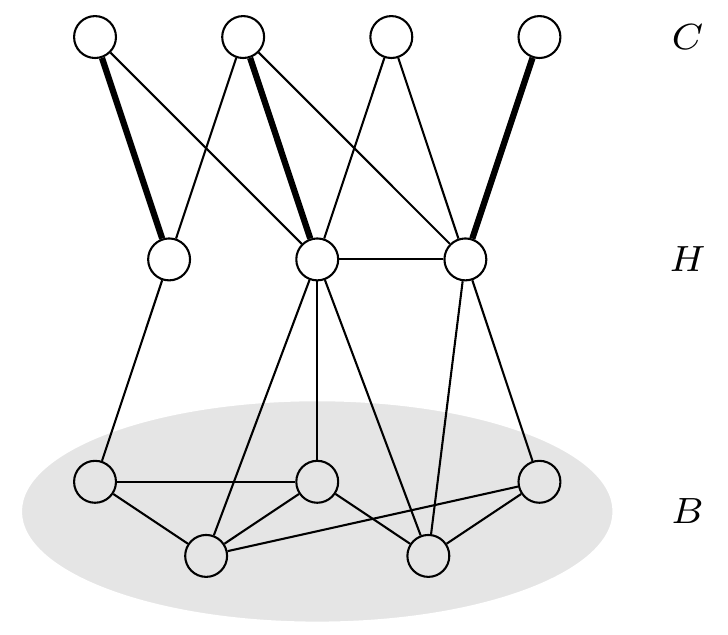
\includegraphics[scale=0.3]{images/crown-decomp.png}
    \caption{Kronenzerlegung: crown, head, body (Quelle: Vorlesung)}
    \label{fig:crown-decomp}
\end{figure}

\paragraph{Satz von König}
Sei $G$ ein ungerichteter bipartiter Graph, sei $M$ ein Matching maximaler Kardinalität,
sei $S$ ein vertex cover minimaler Kardinalität.
Dann gilt $|M| = |S|$.

\underline{Theorem:} $M$ und $S$ können in Polynomzeit berechnet werden.

\paragraph{Lemma}
Sei $G$ ungerichtet, ohne isolierte Knoten, mit $|V| \geq 3k+1$.
Dann existiert ein Polynomzeitalgorithmus der
\begin{enumerate}[label=(\roman*)]
    \item entweder eine Kronenzerlegung berechnet
    \item oder ein Matching $M$ mit $|M| \geq k+1$ findet.
\end{enumerate}
Beweis siehe Buch, Kapitel 6.2, Seite 145f.

\paragraph{Reduktion für VCP} \mbox{} \\
\underline{Lemma:}
Sei $G$ ein Graph mit Kronenzerlegung $V = C \cup H \cup B$ und sei $k \in \N$. Dann gilt: \\
$$ (G, k) \in VCP \iff \Big( G - (C \cup H), k - |H| \Big) \in VCP $$

\underline{Theorem:} Ein Kernbildungsalgorithmus mit obiger Reduktionsregel 
findet einen Kern mit $\leq 3k$ Knoten.


\subsection{Tiefenbeschränkte Suchbäume}

\paragraph{Idee}
Vollständige Suche über alle möglichen Lösungen, aber mit Suchbaumtiefe beschränkt im Parameter.

\paragraph{Beispiel: VCP}
Beobachtung: in jedem vertex cover $S$ gilt $\forall e = \{v_1, v_2\} : v_1 \in S \vee v_2 \in S$.
Daher verzweige von $(G, k)$ nach $(G-\{v_1\}, k-1)$ und $(G-\{v_2\}, k-1)$.
In den Blättern $(G_j, 1)$ ist das VCP trivial.
Dieser Suchbaum hat Tiefe $k$ und $2^{k-1}$ Blätter.
Gesamtlaufzeit: $\bigO (2^k \cdot n)$.

\paragraph{Cluster Editing Problem CEP} \mbox{} \\
Eingabe: Graph $G = (V, E)$, $k \in \N$ \\
Ausgabe: JA falls durch Löschen/Einfügen von $\leq k$ Kanten $G$ in eine Vereinigung (union) von disjunkten Cliquen
(= jeder connected component ist eine Clique) transformiert werden kann, sonst NEIN. \\
Bekannterweise NP-schwer.

\underline{Theorem:}
Graph $G$ besteht aus disjunkten Cliquen \\
$\iff$ $G$ enthält \emph{keinen} Pfad aus drei Knoten\footnote{In eine Clique bilden drei Knoten einen Kreis, keinen Pfad.}\\
$\iff$ es gibt \emph{keine} paarweise verschiedenen $u, v, w \in V : \{u,v\}, \{v,w\} \in E \wedge \{u,w\} \notin E$

\begin{figure}[h]
    \centering
    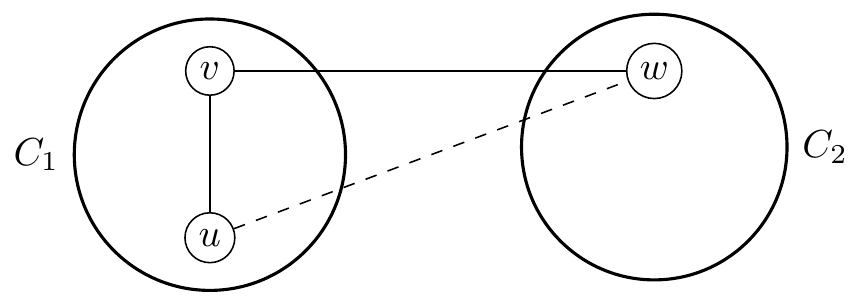
\includegraphics[scale=0.35]{images/cluster-editing.png}
    \caption{Cluster Editing Situation (Quelle: Vorlesung)}
    \label{fig:cluster-editing}
\end{figure}

\underline{Algorithmus:}
Teste ob $G$ bereits eine Vereinigung disjunkter Cliquen ist, oder ob $k=0$.
Wenn nicht, finde $u,v,w \in V$ mit obiger Bedingung.
Rekursiere auf
$G_1 = \big(V, E   -  \{ \{u,v\} \} \big)$,
$G_2 = \big(V, E   -  \{ \{v,w\} \} \big)$,
$G_3 = \big(V, E \cup \{ \{u,w\} \} \big)$.
Laufzeit\footnote{Die Rekursionsformel $T(k) = 3 \cdot T(k-1)$ gibt $\bigO (3^k)$ rekursive Aufrufe.}:
$\bigO (n^3 \cdot 3^k)$.


\subsection{Iterative Kompression}

\paragraph{Idee}
Gegeben ein Kompressionsalgorithmus der aus einer (bzgl. dem Schwellwert) etwas zu grossen Lösung eine kleinere,
gültige Lösung in fpt-Zeit berechnet.
Iteriere: Instanz vergrössern, komprimieren, usw.:
\\
\begin{align*}
(I_0, k_0) & \text{ mit Lösung } S_0^*, |S_0^*| \leq k_0 \\
\xrightarrow{\text{Instanz vergrössern}}
(I_1, k_1) & \text{ mit Lösung } S_1,   |S_1|   > k_1 \\
\xrightarrow{\text{komprimieren}}
(I_1, k_1) & \text{ mit Lösung } S_1^*, |S_1^*| \leq k_1 \\
& \dots
\end{align*}

\paragraph{Disjoint Vertex Cover Problem DVCP} \mbox{} \\
Eingabe: $G=(V,E)$, vertex cover $W$, $k \in \N$ \\
Ausgabe: JA falls es ein vertex cover $S$ gibt mit $|S| \leq k \wedge S \cap W = \emptyset$ sonst NEIN.

\underline{Lemma:}
Jede DVCP-Instanz $(G, W, k)$ kann in Zeit $\bigO (|V|^2)$ gelöst werden (warum?\footnote{
Es reicht zu prüfen ob $N(W)$ ein vertex cover ist}).

\paragraph{Beispiel: VCP}
Idee: füge einen Knoten nach dem anderen hinzu.
Starte mit $S_1^* = \emptyset$. In jeder Iteration setzte $S_i \leftarrow S_{i-1}^* \cup \{v_i\}$ und benutze
$\A_{compress}(G_i, S_i, k)$ um entweder $S_i^*$ zu finden oder NEIN.
Details siehe Buch, Algorithmen 6.6+6.7, Seite 151ff.

\underline{Kompression:} Idee: probiere alle möglichen intersections $X$ des gesuchten VCs mit $S$ aus: \\
If $|S| \leq k$ return $S$.
For all $X \subseteq S$ with $|X| \leq k$ do:
solve DVCP on $(G-X, S-X, k-|X|)$
-- if YES return $X \cup N(S-X)$.
\\
Laufzeit: $\bigO (2^k \cdot n^2)$ also gesamt: $\bigO (2^k \cdot n^3)$.


\subsection{Dynamische Programmierung für den Steinerbaum}

\paragraph{Steinerbaum-Problem STP} \mbox{} \\
Eingabe: $G=(V,E)$ mit Kantenkosten $c : E \mapsto \N$, \emph{Terminalen} $S \subseteq V$,
\emph{Nicht-Terminale/Steiner-Knoten} $N = V-S$ \\
Lösungen: Teilbaum $T$ von $G$ (\emph{``Steinerbaum''}) der alle Knoten aus $S$ enthält (und einige aus $N$) \\
Kosten: $cost(T, (G,c,S)) = c(T) = \sum_{e\in E(T)} c(e) = $ Summe der Kanten = ``Grösse'' des Baums \\
Ziel: $\min$

\paragraph{DP-Ansatz}
Annahme: alle Blätter sind Terminale (warum?).

Beobachtung: falls $Y \subseteq N$ gegeben ist dann ist das STP einfach: berechne MST von $S \cup Y$. \\
$\implies$ k-parametrisierter Algorithmus mit $k = |N|$.

Uninteressant, wir schauen im Folgenden ein DP mit dem Parameter $k = |S|$ an.
Für alle $X \subseteq S$ und alle $v \in V-X$ berechne zwei Steinerbäume:
\begin{enumerate}
    \item Auf Instanz $(G, c, X)$ einen Steinerbaum mit minimalen Kosten $g(X)$.
    \item Auf Instanz $(G, c, X \cup \{v\})$ einen Steinerbaum mit minimalen Kosten $g_{in}(X, v)$ so dass $v$ ein innerer Knoten ist (d.h. $\deg(v) \geq 2$).
\end{enumerate}

\paragraph{Lemma}
Es gilt:
\begin{equation}
g_{in}(X, v) = \min_{\emptyset \neq X' \subset X} \left\{
    g(X' \cup \{v\}) + g \left( (X-X') \cup \{v\} \right)
\right\}
\end{equation}
\begin{equation}
g(X \cup \{v\}) = \min \left\{
    \min_{w \in X} \left\{ p(v,w) + g(X) \right\},
    \min_{w \in V-X} \left\{ p(v,w) + g_{in}(X,w) \right\}
\right\}
\end{equation}
wobei $p(v,w)$ die minimalen Kosten eines Pfades von $v$ nach $w$ in $G$ sind.
Beweis siehe Buch Kapitel 6.5, Seite 159ff.

\paragraph{Dreyfus-Wagner Algorithmus}
Eingabe $(G, c, S)$.
Berechne $p(v, w)$ für alle $v,w \in V$.
Initialisiere $g(\{x,y\}) := p(x,y)$ für alle $x,y \in S$.
Für alle $X \subseteq S$ mit $|X| \in [2, |S|-1]$ und alle $v \in V-X$ berechne $g_{in}(X, v)$ und $g(X \cup \{v\})$.
Gebe $g(S)$ aus.
\\
Laufzeit: $\bigO (n^2 \log n + n \cdot m + (k^2 + )\; 3^k \cdot n + 2^k \cdot n^2)$


\subsection{Baumzerlegung}

\paragraph{Motivation}
Viele schwere Graphprobleme sind auf Bäumen einfach.
Z.B. Reduktionsregel für VCP: entferne Blätter und ihre Nachbarn, füge Nachbarn ins VC hinzu.
\\
Ziel: ``Baumähnlichkeit'' von Graphen beschreiben und ``Baum-Algorithmenvariante'' anwenden.

\paragraph{Definition (Baumzerlegung)}
Eine \emph{Baumzerlegung (tree decomposition)} von $G$ ist ein Paar $D = (T, B)$
wobei $T = (V_T, E_T)$ ein Baum ist.
Sei $I$ eine Indexmenge, die die Knoten aus $V_T$ aufzählt.%
\footnote{Dies erlaubt es uns getrennt über die Knotenmenge $V_T$ des Baums $T$ und über die bags zu sprechen.}
Sei $B$ eine Label-Funktion $B : I \mapsto 2^V$ die jedem Index $i$ von $V_T$ eine Knotenmenge $X_i \subseteq V$
(einen \emph{bag}) zuordnet, so dass:
\begin{enumerate}[label=(\roman*)]
    \item $ \bigcup_{i \in I} X_i = V $ (alle Knoten kommen vor)
    \item $ \forall \{u,v\} \in E \; \exists i \in I : u, v \in X_i $ (alle Kanten in einem bag)
    \item $ \forall v \in V $ bilden die bags $X_i$ mit $v \in X_i$ einen Teilbaum von $T$ (Zusammenhang, Lokalität)
\end{enumerate}

Die \emph{Weite} von $D$ ist $\max \{|X_i|\} - 1$.\footnote{Das $-1$ ist kosmetisch damit echte Bäume eine Baumweite von 1 haben.} \\
Die \emph{Baumweite} $\tw(G)$ von $G$ ist die minimale Weite über alle möglichen Baumzerlegungen.

\begin{figure}[h]
    \centering
    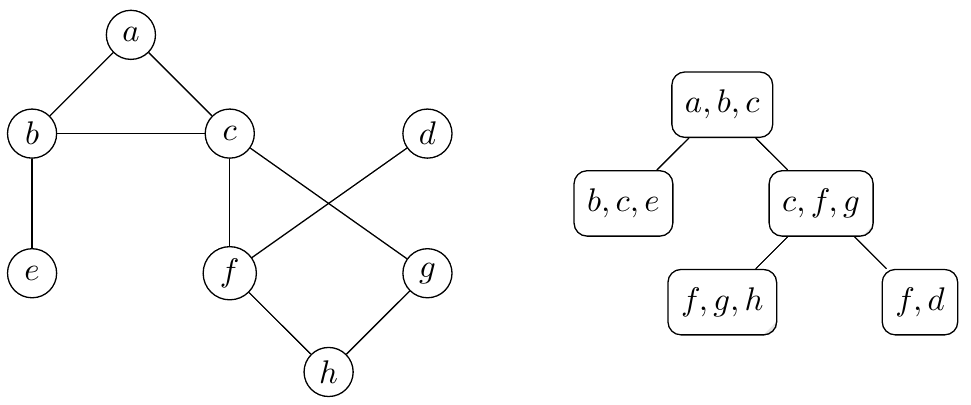
\includegraphics[scale=0.4]{images/tree-decomp.png}
    \caption{Graph $G$ (links) und seine Baumzerlegung $D$ (rechts) (Quelle: Vorlesung)}
    \label{fig:tree-decomp}
\end{figure}

\paragraph{Beobachtungen}
\begin{itemize}
    \item Sei $G$ ein Baum. Dann ist $\tw(G) = 1$.
    \item Sei $G$ ein Kreis. Dann ist $\tw(G) = 2$.
    \item Sei $G$ ein Graph, $v \in V, e \in E$.
    Dann ist jede Baumzerlegung $D$ für $G$ auch eine Baumzerlegung für $G-e$.
    Auch kann $D$ in eine Baumzerlegung $D'$ für $G-v$ transformiert werden mit gleicher oder kleinerer Weite
    (z.B. durch Entfernen von $v$ aus $D$).
    \\
    $\implies$ Die Baumweite ist monoton: zusätzliche Knoten/Kanten verringern nicht die Baumweite.
    \item Sei $G$ ein Graph, sei $C \subseteq V$ eine Clique der Grösse $|C| = k$.
    Dann gilt $\tw(G) \geq k-1$ (und es existiert ein bag, der alle Knoten der Clique enthält).
    \\
    $\implies$ grosse Cliquen $\Rightarrow$ grosse Baumweite.
    ABER kleine Cliquen $\nRightarrow$ kleine Baumweite (z.B. $l \times l$-Gitter-Graph).
    \\
    $\implies$ Konzept der Clique kein genügendes Modell für den Zusammenhang
    (und damit der Baumähnlichkeit) eines Graphen.
    Verallgemeinerung: statt Knoten die sich gegenseitig berühren betrachten wir
    \underline{Mengen von} Knoten die sich gegenseitig berühren.
\end{itemize}

\paragraph{Definition (bramble)}
Sei $G$ ein Graph, sei $\B = \{B_1, \dots, B_k\}$ mit $B_i \subseteq V$
Wir sagen dass $B_i, B_j$ sich \emph{berühren (touch)}, falls
$B_i \cap B_j \neq \emptyset$ oder $\exists \{x_i, x_j\} \in E : x_i \in B_i \wedge x_j \in B_j$.
\\
Wenn alle $B_i$ sich paarweise berühren, dann heisst $\B$ \emph{bramble} (``Dornen-/Brombeergestrüpp'') von $G$.

$C \subseteq V$ heisst \emph{Überdeckung (cover)} von $\B$, falls $C \cap B_i \neq \emptyset$ für alle $i$.
\\
Die \emph{Ordnung (order)} von $\B$ ist die Grösse einer minimalen Überdeckung von $\B$.
\\
Die \emph{bramble number} $\bn(G)$ von $G$ ist die maximale Ordnung eines bramble von $G$.

\underline{Beispiel:}
In einem $k \times k$-Gitter-Graph sei ein ``Kreuz'' $C_{i,j}$ die Vereinigung von Reihe $i$ und Spalte $j$.
Dann ist $\B = \{C_{i,j} \st 1 \leq i,j \leq k \}$ ein bramble von $G$ der Ordnung $k$
und jede Reihe und jede Spalte ist eine Überdeckung von $\B$.

\paragraph{Theoreme}
\begin{itemize}
    \item Sei $G$ ein Graph. Dann gilt $\bn(G) = \tw(G) + 1$. \\
    $\longrightarrow$ Die bramble number beschreibt die Grösse des grössten bags in einer optimalen Baumzerlegung.
    D.h. sie bietet eine untere Schranke für die Weite einer beliebigen Baumzerlegung.
    \item Die Konstruktion einer Baumzerlegung und Bestimmung der Baumweite sind NP-schwer. \\
    $\longrightarrow$ Problem: das Parameter eines parametrisierten Algorithmus' sollte in Polynomzeit berechenbar sein!
    \item Sei $G$ ein Graph mit $\tw(G)=k$. Dann kann man eine Baumzerlegung $D$ der Grösse/Weite $\leq 5k$
    in Zeit $2^{\bigO(k)} \cdot n$ berechnen.
\end{itemize}

\subsubsection{Beispiel: VCP parametrisiert mit Baumweite}

\paragraph{Idee}
Löse VCP in den bags und setze die Gesamtlösung aus den Teillösungen anhand der Baumstruktur bottom-up zusammen.

\paragraph{Definition}
Eine Baumzerlegung heisst \emph{einfach (simple)}, falls $\forall i, j \in I \cl X_i \nsubseteq X_j$.

\paragraph{Lemma}
Jede Baumzerlegung lässt sich umwandeln in eine einfache Baumzerlegung.

\underline{Beweis:}
falls solche $X_i, X_j$ existieren, dann müssen sie auf einem Pfad liegen.
O.B.d.A. ist $X_i$ Nachbar von $X_j$. Kontrahiere beide.
Die Weite bleibt erhalten.
Machbar in Zeit $\bigO(\tw(G) \cdot n)$.\footnote{Wenn die Ausgangszerlegung $D$ wie im Theorem oben gebildet wurde,
impliziert dies dass $D$ $\bigO(n)$ viele bags hat.}

\paragraph{Lemma}
Sei $G$ ein Graph.
Dann existiert eine Baumzerlegung $D=(T,B)$ von $G$ mit (optimaler) Weite $\tw(G)$ so dass $|V_T| \leq |V|$. \\
$\longrightarrow$ Es gibt wenige bags, und diese sind klein.

\underline{Beweis:}
O.B.d.A. hat $D$ Baumweite $\tw(G)$ und ist einfach. Wähle ein $r \in T$ als Wurzel.
$\forall v \in V$ sei $\high(v)$ der höchste Knoten in $V_T$ dessen bag $v$ enthält.
$\high(v)$ ist eindeutig (warum?).
Behauptung: $\forall X_i \exists v \in V \cl \high(v) = X_i$.
Fall nicht, gilt entweder $i = r$, aber dann ist $X_r = \emptyset$.
Oder aber $X_i$ hat einen parent $X_j$, und da es kein eindeutiges $v$ gibt für $X_i$ muss $X_i \subseteq X_j$ gelten.
Beide Fälle sind ein Widerspruch zur Annahme dass $D$ einfach ist.
Also hat jeder bag mind. ein $v$ an höchster Stelle, ergo muss $|V_T| \leq |V|$ gelten.

\paragraph{Notation}
Wurzel $R$, Orientierung von $R$ zu den Blättern.
Teilbaum $T_X$ mit Wurzel $X$.
Induzierter Teilgraph $G[T_X]$ von $G$ mit all den Knoten die in einem bag aus $T_X$ sind.

\paragraph{Definition}
Sei $G$ ein Graph, sei $X \subseteq Y \subseteq V $, seien $C_X, C_Y$ vertex cover für $G[X], G[Y]$.
$C_Y$ \emph{erweitert (extends)} $C_X$, falls $C_X \subseteq C_Y$ \underline{und} $C_Y \cap X = C_X$
(d.h. $C_Y$ stimmt auf $X$ mit $C_X$ überein).

\paragraph{Theorem}
Sei $G$ ein Graph und sei $D$ eine einfache Baumzerlegung von $G$ der Weite $k$.\footnote{$k = \tw(G)$ muss nicht gelten!}
Dann lässt sich ein optimaler VC für $G$ berechnen in Zeit $\bigO (2^k \cdot k \cdot n)$.

\underline{Beweis:} Konstruktiv.
Ziel: verwalte eine Tabelle, die für jeden bag $X$ alle optimalen VCs für $G[T_X]$ enthält -- diese lassen sich
zu einem optimalen VC für $G$ erweitern.
\begin{itemize}
    \item[1)] Initialisierung:
    Für alle bags $X$ berechne alle zulässigen VCs für $G[X]$
    und definiere $w_X : 2^X \mapsto \N \cup \{\infty\}$ für alle $C \subseteq X$ wie folgt:
    $$ w_X (C) = \begin{cases}
    |C| & \text{ if $C$ is a VC for $G[X]$} \\
    \infty & \text{ otherwise}
    \end{cases}$$
    D.h. $w_X$ speichert die Grösse aller VC-Kandidaten für $G[X]$.
    \item[2)] Bottom-up-Durchlauf von $T$:
    Für jeden Knoten $Y$ merge die Information $w_X$ aus jedem seiner Kinder $X$ in $w_Y$ hinein.
    Sobald alle Kinder abgearbeitet sind enthält $w_Y$ die Grösse aller VC-Kandidaten für $G[T_Y]$.

    Merge-Schritt:
    Für alle $C_Y \subseteq Y$, sei $Z = X \cap Y$ und sei $C_Z := (C_Y \cap Z) \subseteq Z$
    (also $C_Y$ erweitert $C_Z$). Dann berechne:
    $$
    w_Y (C_Y) \quad = \quad w_Y (C_Y)
    \quad + \quad \min \{ w_X (C_X) \st C_X \subseteq X \text{ extends } C_Z \} \quad - \quad |C_Z|
    $$
    Beispiel siehe Buch Kapitel 6.6, Seite 173.
\end{itemize}

\underline{Beobachtung:} Jeder Knoten der in $T_X$ aber nicht in $X$ vorkommt, kommt nicht ausserhalb von $T_X$ vor
(wegen Eigenschaft 3 der Baumzerlegung).
Dadurch bleibt die Tabelle klein, da wir für alle abgehandelten ``unteren'' Knoten den optimalen VC bereits kennen.

\underline{Laufzeit:}
\begin{itemize}
    \item[1)] Initialisierung: $2^{k+1}$ Teilmengen pro bag, jede in amortisiert%
    \footnote{Naiv $\bigO (k^2)$ da wir alle Kanten in $G[X]$ auf coverage testen müssen.
    Besser: iteriere über Teilmengen via Gray-Code, so dass sich immer nur ein Knoten ändert,
    d.h. wir nur $\leq k$ Kanten testen müssen.}
    $\bigO (k)$ testbar ob sie ein VC ist.
    $\leq n$ bags (da einfache Zerlegung).
    $\implies \bigO (2^k \cdot k \cdot n)$
    \item[2)] Mergen von $X$ in Vorgänger $Y$:
    Sortiere $w_x$-Tabelle bzgl. Ordnung auf $Z=X \cap Y$ in $\bigO (2^k \cdot \log 2^k)$.
    Finde Minimum für alle $C_Z$ in $\bigO(2^k)$ (da Tabelle sortiert).
    Für jedes $C_Y \subseteq Y$ finde passendes $C_Z$ in $w_x$-Tabelle in $\bigO(\log 2^k)$ dank binärer Suche.
    $\leq n$ merges.
    $\implies \bigO (2^k \cdot k \cdot n)$
\end{itemize}

\paragraph{Korollar}
Das VCP ist fpt bzgl. $\tw(G)$.

\paragraph{[Ausblick] Theorem}
Sei $(G, k)$ eine VCP-Instanz, so dass $G=(V,E)$ planar ist und $|V|=n$.
Dann kann das VCP auf $G$ in subexponentieller Zeit $2^{\bigO (\sqrt{k})} \cdot n$ gelöst werden.

\underline{Beweisidee:}
Berechne einen VC-Kern der Grösse $\bigO (k)$ (insbesondere bleibt der Graph planar).
Ein planarer Graph kann mit Separatoren der Grösse $\bigO (\sqrt{k})$ in Teile der Grösse
$\bigO (\sqrt{k})$ zerlegt werden.
Dann gilt $\tw(G) \in \bigO (\sqrt{k})$ und wir können eine Baumzerlegung mit Weite $\bigO (\sqrt{k})$ finden.
Wende dann den $\tw(G)$-parametrisierten Algorithmus an.


\subsection{Grenzen der Parametrisierbarkeit}

\paragraph{Ziel}
Zeige, dass es Probleme gibt, die keine fpt-Algorithmen erlauben (unter komplexitätstheoretischen Annahmen).

\paragraph{Definition}
Das parametrisierte Problem $(U_1, \Par_1)$ lässt sich auf $(U_2, \Par_2)$ reduzieren mit
\emph{parametrisierter Standardreduktion}, falls es einen Algorithmus gibt, der in fpt-Zeit
Instanzen $(I_1, k)$ in $(I_2, k')$ umwandelt, JA-Instanzen erhält, und $k'$ nur von $k$ abhängt (nicht von $|I_1|$).

\paragraph{Theorem}
Falls $(U_2, \Par_2)$ fpt ist und eine parametrisierte Reduktion von $(U_1, \Par_1)$ auf $(U_2, \Par_2)$ existiert,
dann ist auch $(U_1, \Par_1)$ fpt.

\paragraph{Definitionen}
\begin{itemize}
    \item Das \emph{gewichtete (weighted) 2-SAT Problem (W2SAT)} ist ein parametrisiertes Problem: \\
    Eingabe: 2-KNF Formel $F$, $k \in \N$ \\
    Ausgabe: JA, falls es eine erfüllende Belegung für $F$ mit Gewicht\footnote{Gewicht := Anzahl auf
    1 gesetzter Variablen} genau $k$ gibt. \\
    Parametrisierung: Gewicht $k$
    \item Die Klasse \emph{W[1]} enthält alle parametrisierten Probleme, die sich auf W2SAT parametrisiert
    reduzieren lassen (c.f. Klasse NP).%
    \footnote{Der Name W[1] ist historisch bedingt, die Klasse ist ursprünglich auch nicht via W2SAT definiert.}
    \item Problem $U$ ist \emph{W[1]-schwer}, falls sich W2SAT auf $U$ reduzieren lässt.
    \item Problem $U$ ist \emph{W[1]-vollständig}, falls es in W[1] liegt und W[1]-schwer ist.
    \item Die Klasse \emph{FPT} enthält alle parametrisierten Probleme, für die ein fpt-Algorithmus existiert (c.f. Klasse P).
\end{itemize}

\paragraph{Theorem}
Falls W[1] = FPT, dann kann 3-SAT auf Eingabe $F$ mit $n$ Variablen in Zeit $2^{o(n)} \cdot |F|^{\bigO(1)}$
gelöst werden.

$\longrightarrow$ Schwierigkeit von W[1] steht in direkter Verbindung mit der subexponentieller Lösbarkeit von 3-SAT.
Allerdings: die Bedingung dass ein solcher Algorithmus nicht existiert (\emph{Exponential-Zeit-Hypothese ETH})
ist stärker als P $\neq$ NP (bzw. 3-SAT $\notin$ P).
D.h. W[1]-Vollständigkeit ist schwächer als NP-Vollständigkeit.

\paragraph{Theorem}
Das Independent-Set-Problem ist bzgl. Standardparameter W[1]-vollständig.
